\begin{frame}[fragile]{Algorithms}
Commmon structure:
\begin{small}
\begin{verbatim}
void step(){
    sample_allocations();
    sample_unique_values();
}

void run(BaseCollector* collector){      
    print_startup_message();
    initialize();
    unsigned int iter = 0;
    while(iter < maxiter){
        step();    
        if(iter >= burnin){
            save_state(collector, iter);
        }
    iter++;
    }
    print_ending_message();
}
\end{verbatim}
\end{small}
\end{frame}

\begin{frame}[fragile]{Algoritmhs} %TODO virtual methods in Algorithm
\begin{itemize}
	\item Structure: \texttt{Algorithm<Hierarchy<>, Hypers, Mixture>}
	\item Multivariate data supported
\end{itemize}

\begin{center}
	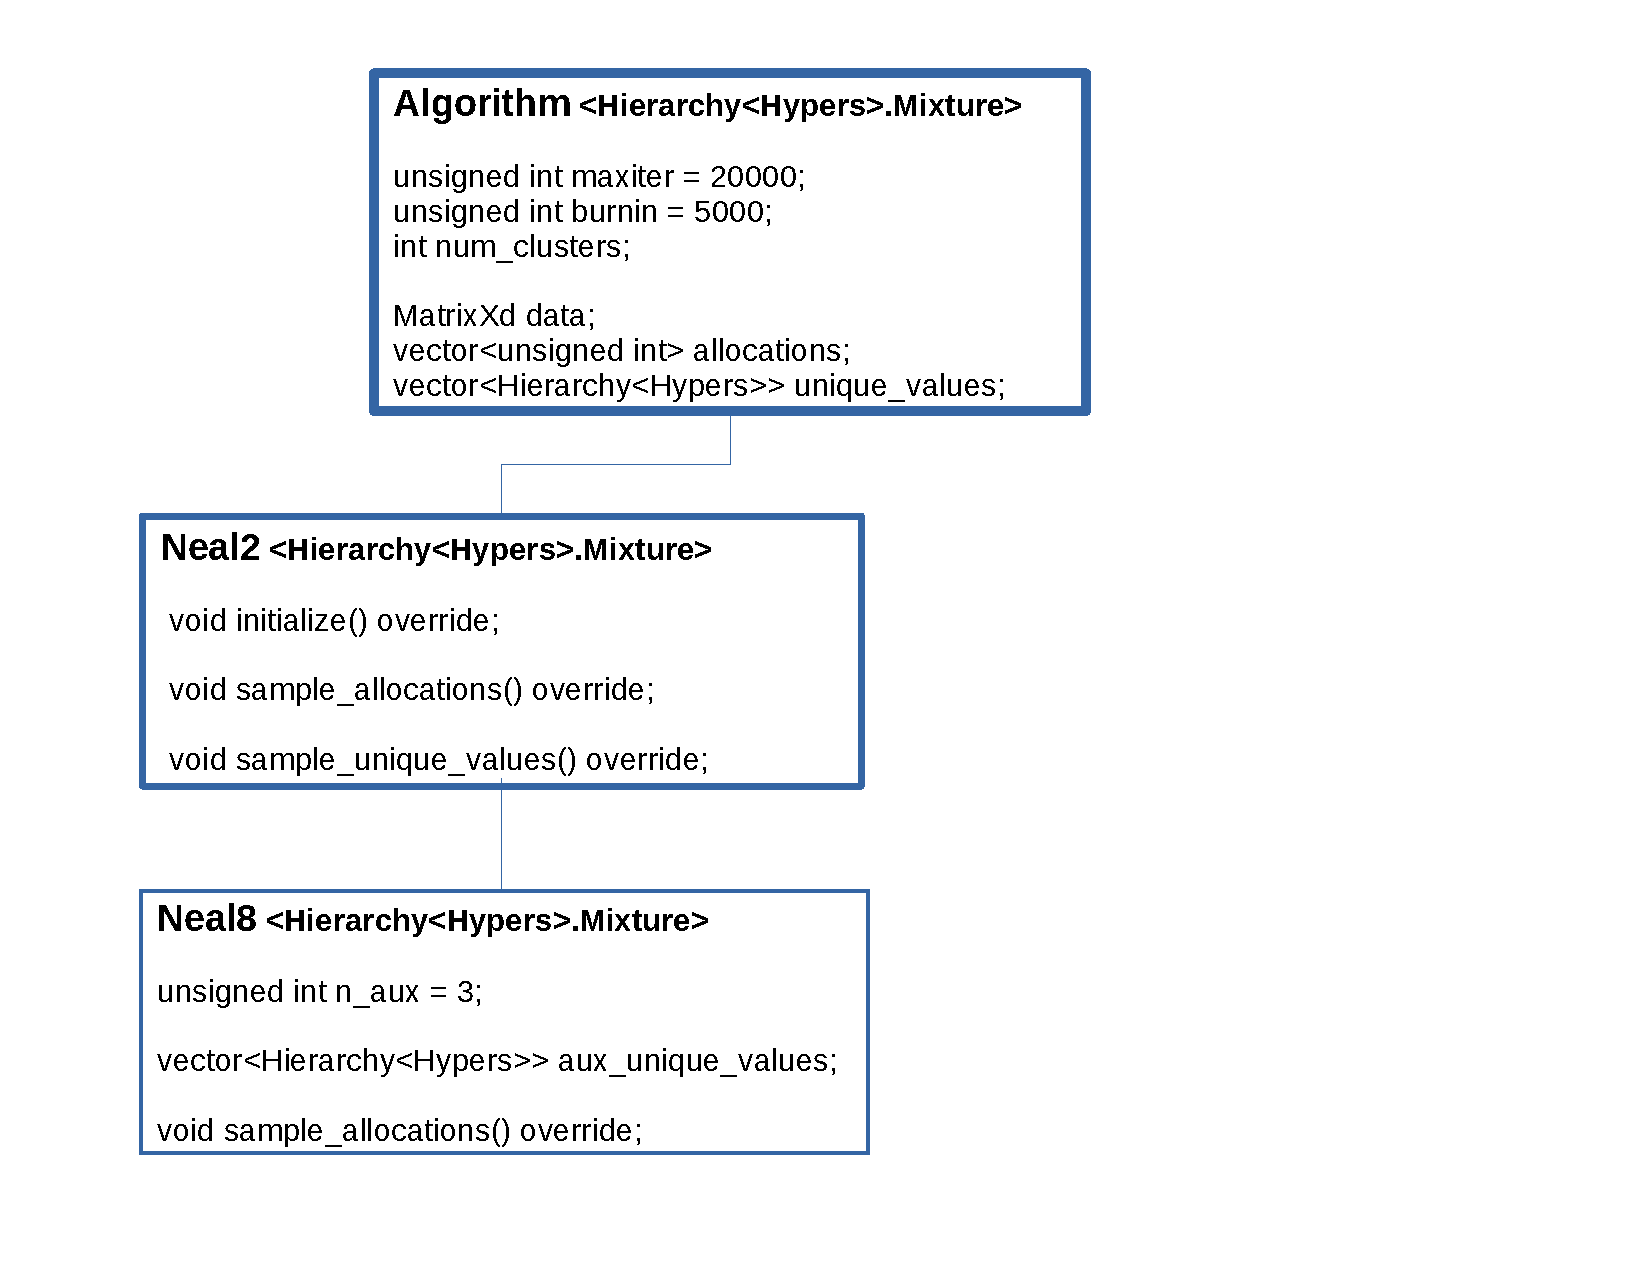
\includegraphics[scale=0.35]{etc/algo.pdf}
\end{center}
\end{frame}


\begin{frame}{Hierarchies (\texttt{Hierarchy})}
\begin{itemize}
	\item Template parameter for \texttt{Algorithm}: common interface needed
\end{itemize}

\begin{center}
	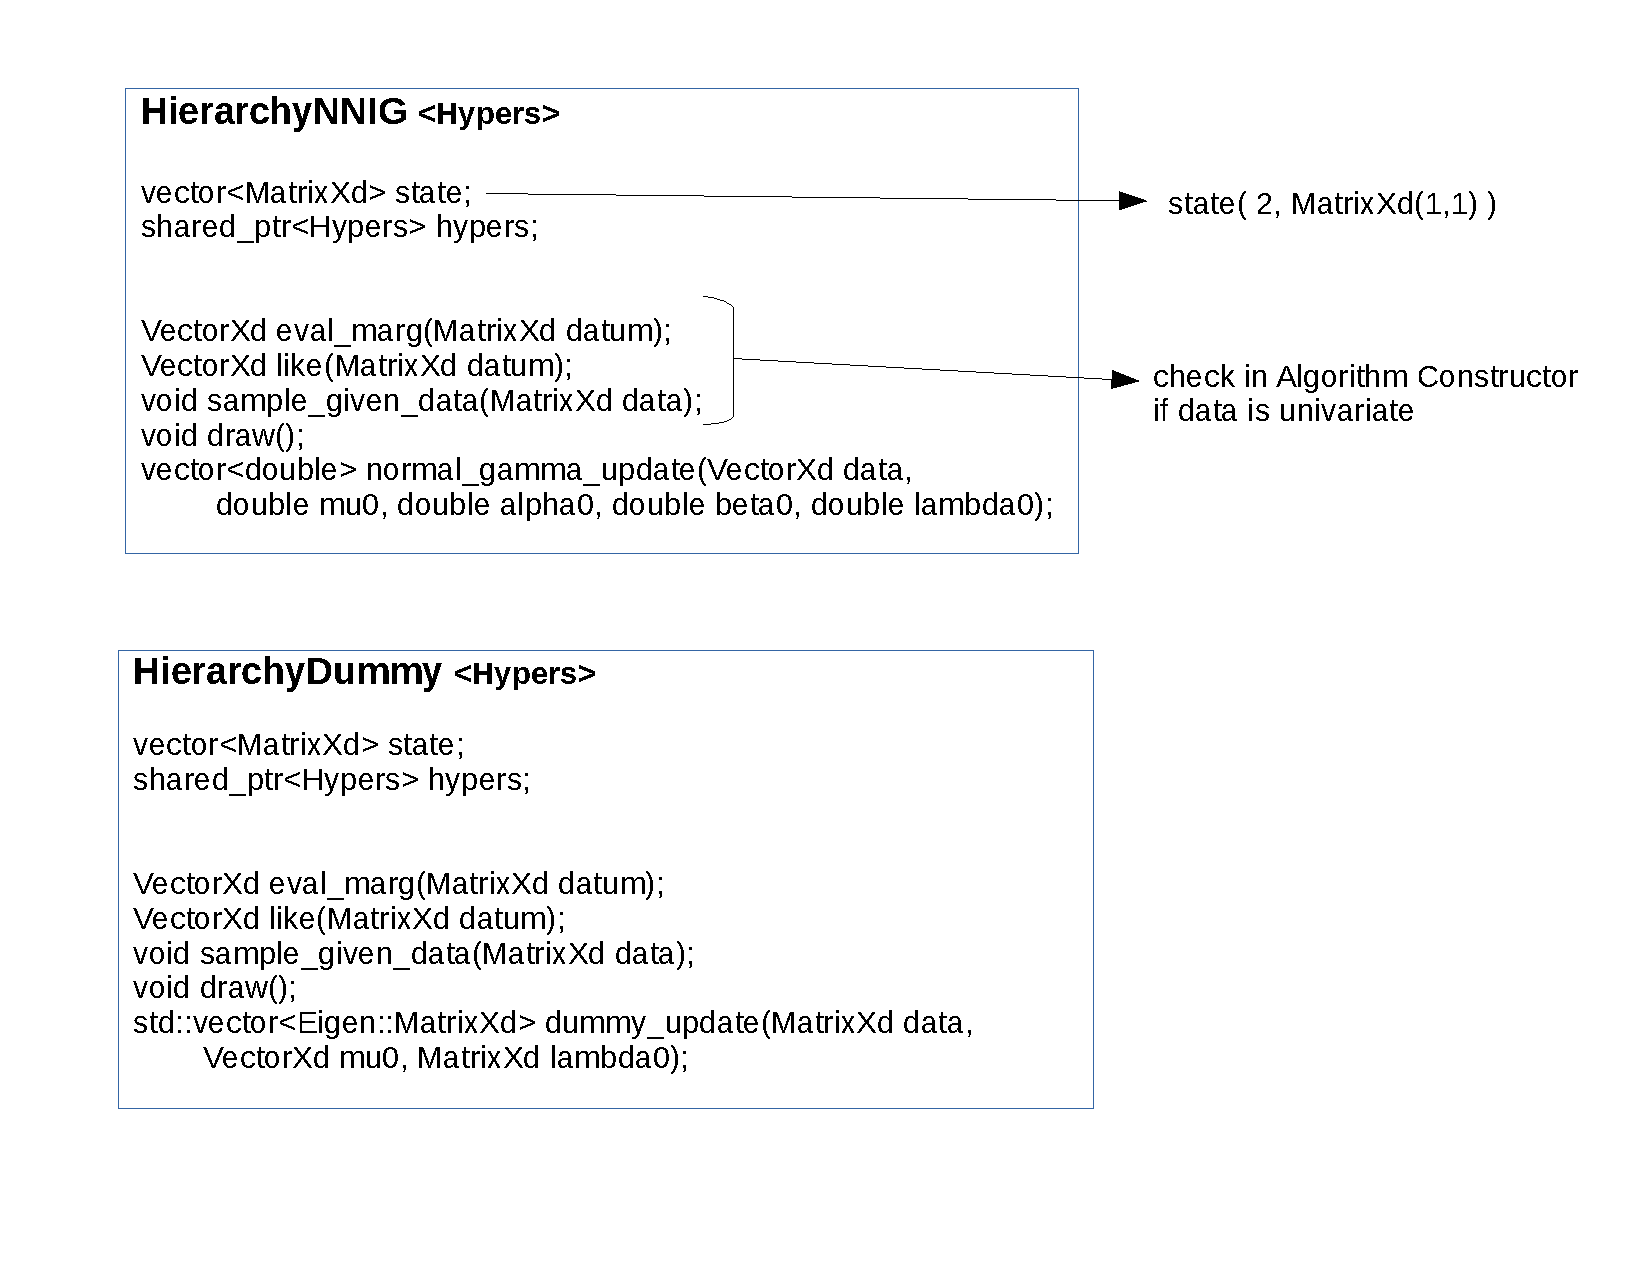
\includegraphics[scale=0.35]{etc/hierarchy.pdf}
\end{center}

\end{frame}


\begin{frame}{Hyperparameters (\texttt{Hypers})}
\begin{itemize}
	\item Template parameter for \texttt{Hierarchy}
	\item Used through a pointer to allow simultaneous update of several hierarchies
\end{itemize}

\begin{center}
	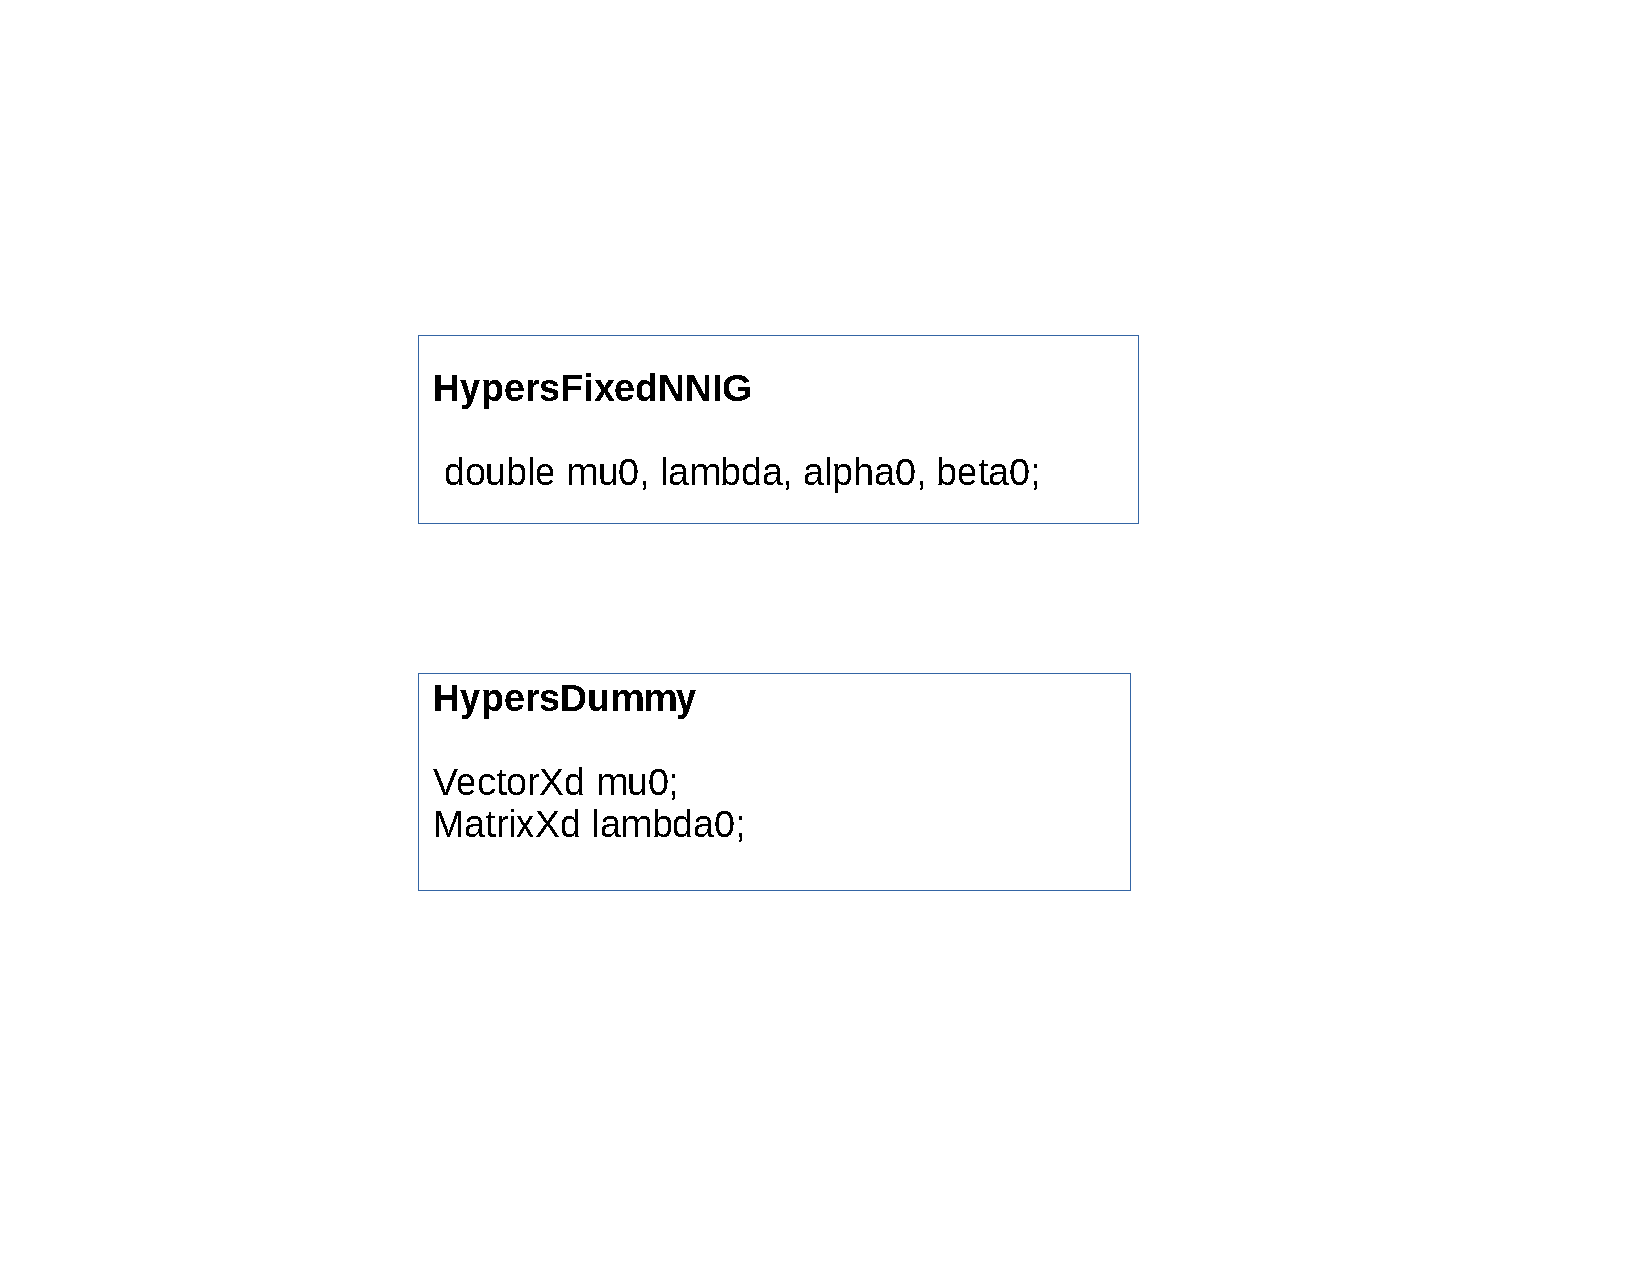
\includegraphics[scale=0.35]{etc/hypers.pdf}
\end{center}
\end{frame}


\begin{frame}{Mixtures (\texttt{Mixture})}
% TODO mancano dei ;
\begin{itemize}
	\item Template parameter for \texttt{Algorithm}: common interface needed
\end{itemize}

\begin{center}
	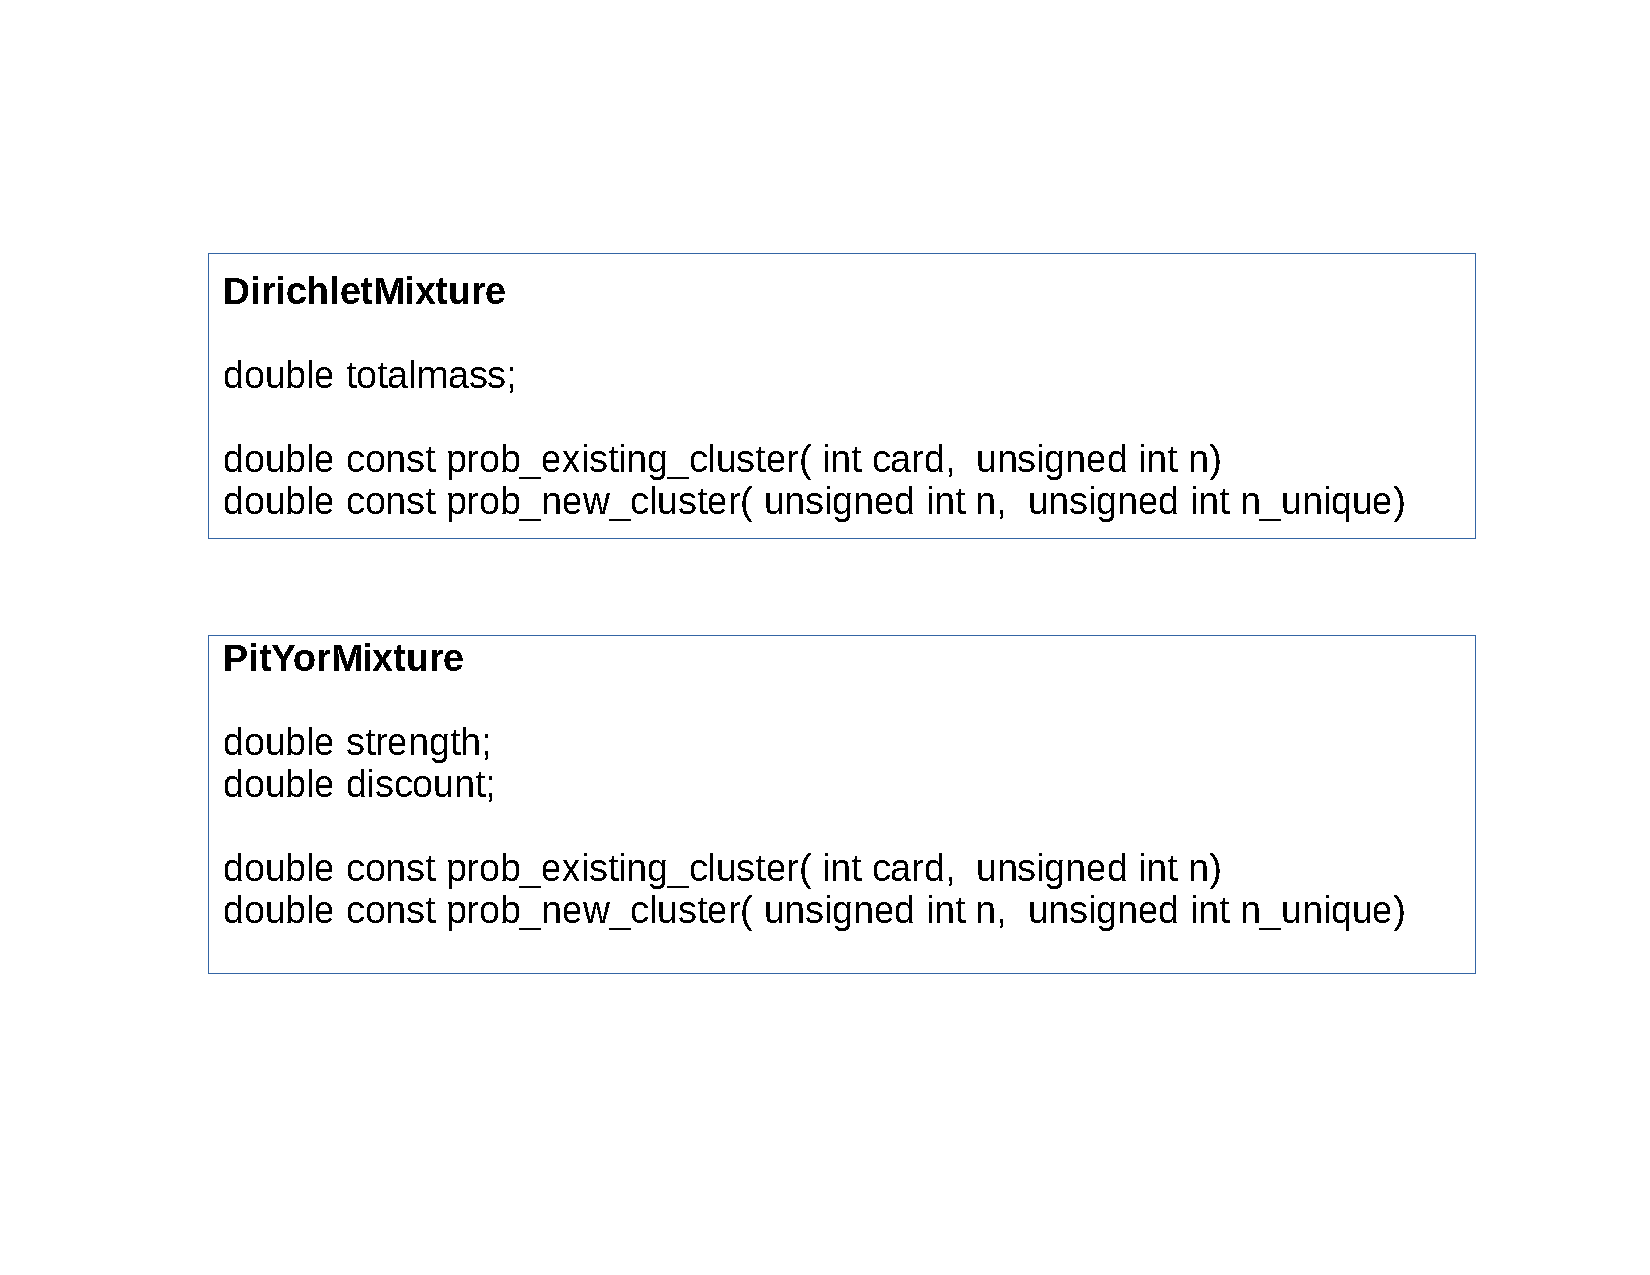
\includegraphics[scale=0.35]{etc/mixture.pdf}
\end{center}

\end{frame}